\documentclass{article}
%\usepackage[austrian]{babel}

\input{epsf}

\usepackage{graphicx}

\usepackage[utf8]{inputenc}
\usepackage{amsmath}

% generic packages needed for math and logic symbols
\usepackage{amssymb}
\usepackage{stmaryrd}
\usepackage{wasysym}
\usepackage{mathrsfs}
\usepackage{array}
\usepackage{xcolor}

%% for logical symbols 
%%% Logical operators
%% Common (but not filtered among those not needed)
\newcommand*{\lnextbase}{\ocircle}
\newcommand*{\lbackbase}{\circleddash}
\newcommand*{\lglobbase}{\square}
\newcommand*{\levenbase}{\Diamond}
\newcommand*{\luntilbase}{\mathbin{\mathcal{U}}}
\newcommand*{\lnextsup}[1]{\mathop{\lnextbase^{#1}}}
\newcommand*{\lbacksup}[1]{\mathop{\lbackbase^{#1}}}
\newcommand*{\lnextsub}[1]{\mathop{\lnextbase_{#1}}}
\newcommand*{\lbacksub}[1]{\mathop{\lbackbase_{#1}}}
\newcommand*{\lnextgen}[2]{\mathop{\lnextbase^{#1}_{#2}}}
\newcommand*{\lbackgen}[2]{\mathop{\lbackbase^{#1}_{#2}}}
\newcommand*{\lguntil}[4]{#3 \mathbin{\mathcal{U}^{#1}_{#2}} #4}
\newcommand*{\luntil}[3]{#2 \mathbin{\mathcal{U}^{#1}} #3}
\newcommand*{\lgsince}[4]{#3 \mathbin{\mathcal{S}^{#1}_{#2}} #4}
\newcommand*{\lsince}[3]{#2 \mathbin{\mathcal{S}^{#1}} #3}
\newcommand*{\lfuntil}[3]{#2 \mathbin{\mathcal{U}(#1)} #3}
\newcommand*{\lglob}[1]{\mathop{\lglobbase^{#1}}}
\newcommand*{\leven}[1]{\mathop{\levenbase^{#1}}}

%% LTL
\newcommand*{\lnext}{\mathop{\lnextbase}}
\newcommand*{\lluntil}[2]{#1 \mathbin{\mathcal{U}} #2}
\newcommand*{\llglob}{\mathop{\lglobbase}}
\newcommand*{\lleven}{\mathop{\levenbase}}

%% probability symbol
\newcommand*{\llprob}{\mathbb{P}}

%for the algorithm showing
\usepackage{algorithm}
\usepackage{algpseudocode}

% to add links to external resources
\usepackage{hyperref}
\hypersetup{
    colorlinks=true,
    linkcolor=blue,
    filecolor=magenta,      
    urlcolor=blue,    
    citecolor=black
}

%to list code in the document
\usepackage{listings}
\usepackage{xcolor}

%% bibliography management
\usepackage[backend=biber,style=numeric,sorting=ydnt]{biblatex}
\addbibresource{biblio.bib} %Import the bibliography file

%% to add todonotes
\usepackage{todonotes}

\newcommand\inParens[1]{\texttt{(}#1\texttt{)}}
\newcommand\inBraces[1]{\texttt{\{}#1\texttt{\}}}
\newcommand\comma{\texttt{,}}
\newcommand\semicolon{\texttt{;}}

\title{Model Checking ``MiniCheck''}

\setlength{\oddsidemargin}{0mm}
\setlength{\evensidemargin}{0mm}
\setlength{\topmargin}{-1cm}
\setlength{\textheight}{22.5cm}
\setlength{\textwidth}{15cm}

%\newcommand{\Nat}{\mbox{I\hspace{-0.1em}N}}
\newcommand{\Nat}{\ifmmode{\sf I\hspace*{-0.3mm}N} \else\mbox{${\sf I\hspace*{-0.3mm}N$}}\fi}
\newcommand{\nat}{\Nat}
\newcommand{\Reell}{\ifmmode{\sf I\hspace*{-0.3mm}R} \else\mbox{${\sf I\hspace*{-0.3mm}R$}}\fi}
\newcommand{\comment}[1]{}
\newcommand{\eqdef}{\mbox{$=_{df}\,$}}

\newcommand{\assnumber}{5}

\pagestyle{empty}

\begin{document}
\large
\thispagestyle{empty}
\begin{center}
  {\Large \textbf{185.A05 Advanced Functional Programming SS 22}}  \\ [1ex] 
            Tuesay, 05/24/2022 \\
               {\Large \textbf{Assignment 5}} \\[.5ex]
              {\Large \textbf{Model Checking Project: MiniCheck}} \\[.5ex]
                 \textbf{All Chapters}  \\ [.75ex]
           \textbf{Topic:} Building a CTL Model Checker plus Implementing a Choice of Modelling/Verification Extensions  \\[1ex]
          \textbf{Submission deadline:} Friday, 06/13/2022, noon (no second submission)  \\ [0.5ex]
          \textbf{Contact:} Samuel Pilz, samuel.pilz@student.tuwien.ac.at, 
                            Francesco Pontiggia, francesco.pontiggia@tuwien.ac.at 
%          (In case of need, this deadline will be extended (details posted via TISS))
\end{center}

\vspace{1ex}
\noindent
\noindent

\newcommand{\code}[1]{\texttt{#1}}

\noindent
The goal of the project is to implement a  Model Checker, \textit{MiniCheck}, 
for the so called Computational Tree Logic (CTL). 
The project consists of two parts: the core model checker and 
the elective modular extensions. 

\paragraph{Part I - The MiniCheck Core.} The core model checker requires: 
\begin{itemize}
    \item a number of preliminary programming tasks dealing with Transition Systems (TS)
          and Computational Tree Logic (CTL) (cf.~Section \ref{subsec-ts} and \ref{subsec-ctl}).
    \item a verification module which checks an input CTL formula on a TS (cf.~Section \ref{subsec:mc}).
    \item a test suite allowing to validate the usability and correctness of the
          various components of the core (cf.~Section \ref{subsec-testsuite}).
\end{itemize}  
An illustrating example highlights the essence of model-checking in our setting (cf.~Section \ref{subsec:example}). Note that the core is mandatory but is only worth a portion of the points achievable in this project. To achieve the full amount of points some of the extensions have to be chosen and implemented, too.

\paragraph{Part II - The MiniCheck Extensions.} The extensions of the MiniCheck core concern 
\begin{itemize}
    \item software model checking (cf.~Section \ref{sec:ext1})
    \item bounded linear time logic model-checking (cf.~Section \ref{sec:ext2})
\end{itemize}
Each extension is worth the shown amount of points. Note that none of the described extensions are necessary for a positive grade. Additionally, there is a bonus task allowing to achieve even more than the full amount of points for the project (cf.~Section \ref{sec-bonus}). 
\bigskip

In Section \ref{sec:artefacts}, finally, the submission artefacts are detailed. In contrast to previous assignments, you are not asked to implement functions with given signatures. 
Instead, the functionality of the executed program is evaluated. 
You will have to design your own function signatures and data types and decide 
which data structures you want to use.

The program should not be written in a single file, but as a \href{https://docs.haskellstack.org/en/stable/README/}{\code{stack}} 
or \href{https://cabal.readthedocs.io/en/3.4/}{\code{cabal}} project consisting of multiple modules. 
It is encouraged to use custom and predefined data structures, as well as external libraries 
and Haskell language extensions \textbf{where appropriate}. It is not required to get the project to run on g0.

There will be a Q\&A session where help will be provided in case there are troubles with the selected technologies. 
The date will be announced via TUWEL news.

\section{Grading}

The preliminary programming tasks with two parsers at its core (cf.~Section \ref{subsec-ts} and \ref{subsec-ctl}), the verification module (cf.~Section \ref{subsec:mc}) 
and the test suite (cf.~Section \ref{subsec-testsuite}) of MiniCheck are mandatory. 
Implementing this core awards up to 200 points. The project presentation will be worth up to 100 points. 
To gain more points on top of the aforementioned, you can choose from some modelling 
and verification extensions of the MiniCheck tool (cf.~Section \ref{sec:ext1} and \ref{sec:ext2}) and the bonus task (cf.~Section \ref{sec-bonus}).

For a positive evaluation of this project at least 200 points are required. 
A positive grade on the project is necessary in order to receive a positive grade in this course. 

The total points for the project are calculated by adding up the points on the core, 
the selected extensions and the submission talk. A positive grade on the core itself is \textit{not} required. 
At most 300 points are awarded for the project implementation.

In contrast to previous exercises, there is no second submission.

\subsection{Note}
We assume a general knowledge of model checking and its purpose, as well as basis of logics,
such as propositional logic.  Besides this, some previous knowledge in related fields helps 
and makes the project smaller, but it's not mandatory. This includes also:
\begin{itemize}
    \item Automata Theory
    \item Graph Algorithms
\end{itemize}
See, e.g., \cite{BaKa} for details (a PDF version is available on the 
\href{https://github.com/francescopont/MiniCheck.git}{Github repository}).

\section{MiniCheck Core (200 P)}

Model Checking consists of formally and exhaustively verifying a formula 
against all the possible executions of a particular type of automata. 
In the following, we provide some preliminary information 
about the type of the formalisms you are required to support, 
and then present the project to carry out. 
For a complete and deeper introduction to our approach in model checking, 
please, refer to \cite{BaKa}.


\subsection{Preliminaries - Transition Systems}
\label{subsec-ts}
As modelling formalism, we use \emph{Transition Systems} (TS). They are a particular variant 
of Finite State Automata which allow to describe adequately both hardware and software systems. 
They are defined over infinite runs, and they do not have a set of final states. 
Formally, a TS is a tuple ($S, Act, \rightarrow, I, AP, L$), where 
\begin{itemize}
    \item $S$ is a set of \emph{states},
    \item $Act$ is a set of \emph{actions},
    \item $\longrightarrow\,\subseteq S \times Act \times S$ is a \emph{transition relation},
    \item $I \subseteq S$ is a set of \emph{initial states}.
    \item $AP$ is a set of \emph{atomic propositions}, and 
    \item $L : S \rightarrow 2^{AP}$ is a \emph{labelling function}.
\end{itemize}
Actions are used to specify how the system evolves from one state to another. The labelling function maps every state to the set of atomic propositions holding in that state. The initial state is chosen nondeterministically between all states $\in I$.
We adopt a \textbf{state-based} approach: we consider (and want to verify) the labels in the state sequence of a run of the TS, and abstract from actions, which are of no use in our verification algorithm. 

Note that, for simplicity sake, we consider only TS with no terminal states, i.e., every state has at least one outgoing edge. While this prevents some technical problems from occurring, it is not a limit to the expressive power of TS: for every state $s$ without outgoing edge, you can get rid of terminal states by defining a transition to a sink state $s_ {sink}$, and then define a self transition from $s_ {sink}$ to itself.

\subsubsection*{Resources}
\cite[Paragraph 2.1]{BaKa}

\subsubsection*{Task 1}
Define:
\begin{itemize}
    \item a suitable plain-text representation of TS such that TS written in this representation
          can be passed as input to your tool, and
    \item a data type to represent them. 
    \item the type of the set of atomic propositions that can be used to label states of the           Transition System.These are usually either a description of the state (e.g., OFF for a         system that describes a lightbulb) or a property that holds in the state (e.g. $nsoda == 0$     for a system that describes the functioning of a soda vending machine). We refer to  the       example in Section \ref{subsec:example}.
\end{itemize} 
Implement: 
\begin{itemize}
    \item A parsing function from the plain-text representation of TS to the data type.
\end{itemize}
Take care of making sure that there are no terminal states, that there is at least an initial state, and that your formalisation of the set of atomic propositions is respected. The parsing function should abort when it encounters a non well-formed Transition System.

You are allowed to choose one of the parsing approaches presented in the lecture or 
use an external monadic parsing library from Hackage. Document your choice.

We require that a state is always labelled with itself 
(i.e., $s_i \in L(s_i)$, which implies $S \subset AP$). This does not mean that the atomic propositions we are considering are only state identifiers. As introduced earlier, a state may be labelled with different types of properties depending on the context: it will be up to you to define a suitable type to make your program be able to encode and deal with as many different situations as possible.

\subsection{Preliminaries - Computational Tree Logic}
\label{subsec-ctl}
To express properties to verify on Transition Systems, we consider a temporal extension of propositional logic, i.e., the introduction of temporal modalities on top of propositional logic. 

In particular, the temporal modalities we consider are $\ocircle$ (pronounced ``next'') and $\luntilbase$ (pronounced ``until'').
These temporal modalities allow to constrain the future states (or, in fact, their labels), that can be visited by a path.

Moreover, CTL (differently with respect to some other logics, e.g. LTL) is based on a \emph{branching} notion of time. With this approach, future time corresponds to an infinite tree of states than can be visited after the current one. In fact, branching time refers to the fact that at each moment there may be several different possible futures. By fixing a choice of a state at every subtree, we get one of all \emph{possible} futures. 
Each traversal of the tree starting in its root represent a single path. The tree rooted at state $s$ thus represents all possible infinite computations in the transition system that start in $s$.

Computation Tree Logic (CTL) thus allows to express properties for \emph{some} or \emph{all} computations that start in a state. For this purpose, it features two operators: an existential path quantifier ($\exists$) and a universal path quantifier ($\forall$). Intuitively, $\exists \varphi$ holds in a state if there exists \emph{some} path satisfying $\varphi$ that starts in that state. Dually, $\forall \varphi$ holds in a state if \emph{all} states starting in that state satisfy $\varphi$.

The atomic proposition $a \in AP$ stands for the state label $a$ in a TS.

\subsubsection*{CTL Syntax}
Given a set $AP$ of atomic propositions, with $a \in AP$, CTL formulae follow the following syntax: 
\begin{align*}
    \emph{(state) formulae } & \Phi ::= \text{true} \mid a \mid \Phi_1 \land \Phi_2 \mid \neg \Phi \mid \exists \varphi \mid \forall \varphi \\
    \emph{path formulae   }    & \varphi ::= \lnext{\Phi} \mid \lluntil{\Phi_1}{\Phi_2} \\
\end{align*}
Greek capital letters denote CTL (state) formulae, whereas lowercase Greek letters denote CTL path formulae. 
A well defined CTL formula is a CTL state formula.

In addition, we introduce the following \emph{derived} Boolean operators for state formulae: 
\begin{align*}
    &\; \Phi_1 \lor \Phi_2 \equiv \neg (\neg \Phi_1 \land \Phi_2) \\
    &\; \Phi_1 \rightarrow \Phi_2 \equiv \neg \Phi_1 \lor \Phi_2 \\
    &\; \Phi_1 \leftrightarrow  \Phi_2 \equiv (\Phi_1 \rightarrow \Phi_2) \land (\Phi_2 \rightarrow \Phi_1) \\
    &\; \Phi_1 \oplus  \Phi_2 \equiv (\Phi_1 \land \neg \Phi_2) \lor (\Phi_2 \land \neg \Phi_1)\\
\end{align*}

Likewise, we derive some well-known temporal modalities for path formulae: 
\begin{itemize}
    \item $\lleven$ (pronounced ``eventually''), and
    \item $\llglob$ (pronounced``generally/always");
\end{itemize}

These operators can be derived from the base operators through the following
\begin{align*}
    &\; \exists \lleven \Phi \equiv \exists(\lluntil{\text{true}}{\Phi}) \\ 
    &\; \forall \lleven \Phi \equiv \forall(\lluntil{\text{true}}{\Phi}) \\ 
    &\; \\ 
    &\; \exists \llglob \Phi \equiv \neg\forall \lleven \neg\Phi \\ 
    &\; \forall \llglob \Phi \equiv \neg\exists \lleven \neg\Phi \\
\end{align*}

You are required to handle all and only these operators (this excludes the weak until operator, for example).

\subsubsection*{Hint about derived operators}
If your code translates formulae with derived operators into formulae 
with only base operators through these equivalence rules, you will have implemented support of 
derived operators for free (even if performances will suffer).

\subsubsection*{CTL Semantics}
Given atomic proposition $a \in AP$, $TS = (S, Act, \rightarrow, I, AP, L)$, state $s \in S$, CTL state formulae $\Phi, \Psi$, CTL path formula $\varphi$, the semantics of CTL is defined in terms of the following satisfaction relation $\vDash$ (pronounced ``satisfies") for state $s$. We recall that $s \vDash \Phi$ if and only if $\Phi$ holds in $s$.
\begin{align*}
     & \sigma \vDash \text{true} & \\
     & \sigma \vDash a &\; \text{ iff } & a \in L(s) \\ 
     & \sigma \vDash \neg \Phi &\; \text{ iff } & \text{not } s \vDash \Phi \\
     & \sigma \vDash \Phi \land \Psi & \text{ iff }&  (s \vDash \Phi) \text{ and } (s \vDash \Psi) \\
     & \sigma \vDash \exists \varphi & \text{ iff } & \pi \vDash \varphi \text{ for some } \pi \in Paths(s) \\ 
     & \sigma \vDash \forall \varphi & \text{ iff }& \pi \vDash \varphi \text{ for all } \pi \in Paths(s) \\ 
\end{align*}

Given a path $\pi$, $\vDash$ is defined for path formulae as follows: 
\begin{align*}
    & \pi \vDash \lnext{\Phi} & \text{ iff } \pi[1]  \vDash \Phi \\ 
    & \pi \vDash \lluntil{\Phi}{\Psi} & \text{ iff } \exists j \geqslant 0. (\pi[j]  \vDash \Psi \land (\forall 0 \leqslant k < j. \pi[k]  \vDash \Phi))
\end{align*}

A TS satisfies CTL formula $\Phi$ if and only if $\Phi$ holds for all initial states.

\subsubsection*{Task}
Define:
\begin{itemize}
    \item a suitable plain-text representation of CTL formulae such that formulae written in this representation can be passed as input to your tool, and 
    \item a data type to represent them.
    \item the type of the set of atomic propositions ($APs$) that can be used in the formulae (the same reasoning for LTL $APs$ applies).
\end{itemize}

\subsubsection*{Task}
It is up to you to decide how to combine the two plain text representations of the inputs (the TS and the formula), and how to provide them to the Model Checker via some command-line arguments. Any potential issue with command line arguments must be treated adequately (e.g., missing arguments, too many arguments, wrong arguments, \dots).

The results of a model check query should be printed on the CLI (command line interface), together with some additional information you find useful.

\subsubsection*{Resources}
\cite[Paragraph 6.2 (in particular 6.1.1 and 6.1.2)]{BaKa}

\subsection{The Model Checking procedure}
\label{subsec:mc}
The model checking procedure for CTL formulae differs completely from automata-based procedures, like in LTL verification. It's essentially a bottom-up traversal of the parse tree of the formula at hand, and it is considered way more efficient and straightforward, since it does not involve any notion of corresponding automaton for the input formula. Instead, given a TS and a CTL formula $\Phi$, to verify whether TS $\vDash \Phi$, we establish whether $\Phi$ is valid in each initial state $s$ of TS directly using $s$ and TD. 
Therefore, the procedure is roughly composed of two steps: 
\begin{itemize}
    \item computing the set $Sat(\Phi)$ of all states satisfying $\Phi$ (recursively), and
    \item checking whether all initial states $s \in I$ belong to $Sat(\Phi)$; 
\end{itemize}
In other words, TS $\vDash \Phi$ if and only if $I_{TS} \subseteq Sat(\Phi)$.

\subsubsection{Remark about the notation}
In the following, we present a procedure which computes the satisfaction sets for formulae of 
CTL expressed in the so called \emph{existential normal form}(ENF). This form is the smallest subset of CTL formulae that preserves the same expressive power of full CTL. In other words, for each CTL formula, there exists an equivalent CTL formula expressed in ENF. The set of formulae in ENF is given by: 
\begin{align*}
    & \Phi ::= \text{true} \mid a \mid \Phi_1 \land \Phi_2 \mid \neg \Phi \mid \exists \lnext{\varphi} \mid \exists (\lluntil{\Phi_1}{\Phi_2} \mid \exists \llglob \Phi \\
\end{align*}
We see that the $\forall$ operator is not present in CTL formulae in ENF.
Again, you can either define by yourself the satisfaction set for all CTL formulae, or you can sacrify performances and translate the remaining formulae in EFN (which is the easier way).
The translation rules can be found in \cite[Paragraph 6.2.4]{BaKa}:
\begin{align*}
    & \forall \lnext{\Phi} & \equiv & \text{ } \neg \exists \lnext{\neg \Phi} \\
    & \forall \big( \lluntil{\Phi}{\Psi} \big) & \text{ } \equiv & \neg \exists \big( \lluntil{\neg \Psi}{(\neg \Phi \land \neg \Psi)} \big) \land \neg \exists \llglob \neg \Psi \\
\end{align*}
For derived temporal operators, one can use:
\begin{align*}
    & \exists \lleven \Phi & \equiv & \text{ } \exists \big(\lluntil{\text{true}}{\Phi}\big) \\
    & \forall \lleven \Phi & \equiv  & \text{ }\neg \exists \llglob \neg \Phi \\ 
    & \forall \llglob \Phi & \equiv & \text{ } \neg \exists \lleven \neg \Phi \equiv \neg \exists \big(\lluntil{\text{true}}{\neg \Phi} \big) \\
\end{align*}

\subsubsection{The algorithm}
The following algorithm sketches the procedure. 
\label{subsec-CTLmca}
\begin{algorithm}[H]
    \caption{CTL Model Checking}
    \hspace*{\algorithmicindent} \emph{Input}: finite transition system TS and CTL formula $\Phi$ (both over $AP$) \\
    \hspace*{\algorithmicindent} \emph{Output}: ``yes'' if $TS \vDash \Phi$; otherwise, ``no''
    \begin{algorithmic}[1]
    \Function{$SatFun$}{$\phi$}
        \If{$\phi$ contains state subformulae}
            \State // for children nodes $\psi_1, \psi_2$ of the parse tree of $\phi$, the so called \emph{maximal proper subformulae}
            \State $Sat(\psi_1) = SatFun(\psi_1)$; $Sat(\psi_2) = SatFun(\psi_2)$ 
            \State combine $Sat(\psi_1), Sat(\psi_2)$ depending on the operator of $\phi$ ($\land, \exists\lnext, \exists\mathbin{\mathcal{U}}, \exists\llglob$).
        \Else
            \State compute directly the set $Sat(\phi)$.
        \EndIf
        \State return $Sat(\phi)$.
    \EndFunction
    \State return $I \subseteq Sat(\Phi)$.
    \end{algorithmic}
\end{algorithm}

\subsubsection*{Characterization of $Sat(\cdot)$ for CTL formulae in ENF}
We now formally define the set $Sat(\cdot)$ for every formula, possibly depending on the satisfaction set of subformulae. Let TS $ = (S, Act, \rightarrow, I, AP, L)$ be a transition system without terminal states. For all CTL formulae $\Phi$, $\Psi$ over $AP$ it holds:
\begin{align*}
    & Sat(\text{true}) := S \\
    & Sat(a) := \{ s \in S \mid a \in L(s) \}, \text{ for any a } \in AP \\ 
    & Sat( \Phi \land \Psi) := Sat(\Phi) \cap Sat(\Psi) \\ 
    & Sat(\neg \Phi) := S \setminus Sat(\Phi) \\ 
    & Sat(\exists \lnext{\Phi}) := \{ s \in S \mid Post(s) \cap Sat(\Phi) \neq \varnothing \\
    & Sat\big(\exists (\lluntil{\Phi}{\Psi}) \big) \text{ is the smallest subset T of S such that}: \\
    & \text{   (1)   } Sat(\Psi) \subseteq T \text{ and (2) } s \in Sat(\Phi) \text{ and } Post(s) \cap T \neq \varnothing \text{ implies } s \in T \\
    & Sat(\exists \llglob \Phi) \text{is the largest subset T of S, such that }\\
    & \text{   (3)   } T \subseteq Sat(\Phi) \text{ and } (4) s \in T \text{ implies } Post(s) \cap T \neq \varnothing \\
\end{align*}
where
\begin{align*}
    Post(s) := \bigcup_{\alpha \in Act} \{ s^{'} \in S \mid s \xrightarrow{\alpha} s^{'} \}
\end{align*}
is just the set of successors of a state.

\subsubsection{How to compute $Sat(\cdot)$}
For most cases, you can just stick to the definition. There are only two critical situations.
To compute $Sat\big(\exists (\lluntil{\Phi}{\Psi}) \big)$ and $Sat(\exists \llglob \Phi)$, an iterative approach is required to compute respectively the smallest subset and the greatest subset that verify the property. The two algorithms are sketched here.

\begin{algorithm}[H]
    \caption{Computation of the satisfaction set for Until formulae}
    \hspace*{\algorithmicindent} \emph{Input}: finite transition system TS with state set S and CTL formula $\Phi_1 := \exists (\lluntil{\Phi}{\Psi})$ (both over $AP$) \\
    \hspace*{\algorithmicindent} \emph{Output}: $Sat(\Phi_1) = \{ s \in S \mid s \vDash \Phi_1 \}$
    \begin{algorithmic}[1]
        \State T := $Sat(\Psi)$; (* compute the smallest fixpoint *)
        \While { $\{ s \in Sat(\Phi) \setminus T \mid Post(s) \cap T \neq \varnothing \} \neq \varnothing $}
            \State $ T := T \cup \{ s \in Sat(\Phi) \setminus T \mid Post(s) \cap T \neq \varnothing \} $;
        \EndWhile
    \State return T;
    \end{algorithmic}
\end{algorithm}
\subsubsection{Resources}
\cite[Paragraph 6.4]{BaKa}

\begin{algorithm}[H]
    \caption{Computation of the satisfaction set for Existential Always formulae}
    \hspace*{\algorithmicindent} \emph{Input}: finite transition system TS with state set S and CTL formula $\Phi_1 := \exists (\llglob \Phi)$ (both over $AP$) \\
    \hspace*{\algorithmicindent} \emph{Output}: $Sat(\Phi_1) = \{ s \in S \mid s \vDash \Phi_1  \}$
    \begin{algorithmic}[1]
        \State T := $Sat(\Phi)$; (* compute the greatest fixpoint *)
        \While { $\{ s \in T \mid Post(s) \cap T = \varnothing \} \neq \varnothing$ }
            \State $ T := T \cup \{ s \in T \mid Post(s) \cap T = \varnothing \} $;
        \EndWhile
    \State return T;
    \end{algorithmic}
\end{algorithm}
\subsubsection{Resources}
\cite[Paragraph 6.4]{BaKa}

\subsubsection*{Task}
Implement the model checking algorithm presented here.

\subsection{Test Suite}
\label{subsec-testsuite}
Projects of this size profit from an automatic test-suite. 
Write a test-suite for the major components of the project using one of the following frameworks:

\begin{itemize}
\item \href{https://hackage.haskell.org/package/hspec}{\texttt{hspec}}, a tutorial can be found \href{https://hspec.github.io/}{\texttt{here}}
\item \href{https://hackage.haskell.org/package/tasty}{\texttt{tasty}}
\item \href{https://hackage.haskell.org/package/HTF}{\texttt{HTF}}
\item \href{https://hackage.haskell.org/package/HUnit}{\texttt{HUnit}}
\end{itemize}

As before, it is encouraged to utilise external libraries for writing tests.

It is required to write at least three unit tests for the components of
Section \ref{subsec-ts} and \ref{subsec-ctl}, and a test unit for the
components of Section \ref{subsec:mc}.

\subsection{Example} \label{subsec:example}
We give now an example of a Transition System and some formulae that hold for it. The example has been taken from \cite[Paragraph 2.1]{BaKa}.
The following picture represents a preliminary design of a beverage vending machine. The machine can either deliver beer or soda. States are indicated by ovals and transitions by labelled edges. Every state is labelled with some description of the state itself. Initial states are indicated by having an incoming arrow without source.
\begin{figure}[H]
  \begin{center}
      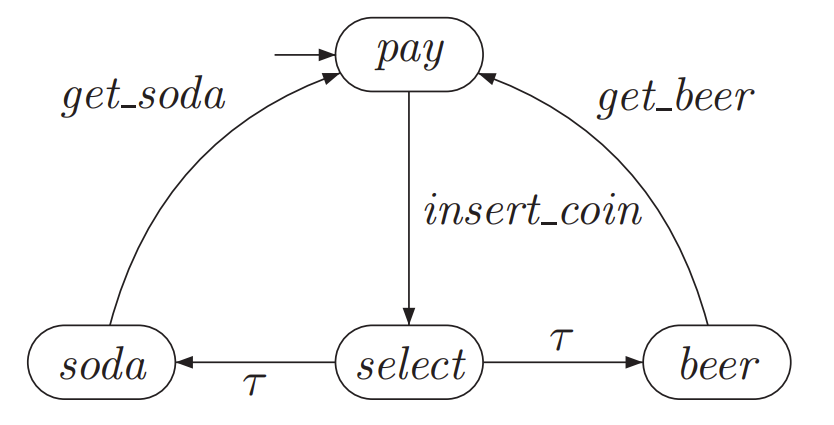
\includegraphics[scale = 0.50]{pictures/example.png}
  \end{center}
\end{figure}
The following formulae hold for this TS (note, $\tau$ denotes an internal transition of the TS):
\begin{itemize}
    \item $\{ \forall \lleven  \text{pay} \}$ := every path will eventually return to the initial state, which is labelled with ``pay'';
    \item $\{ \exists \lleven \text{ soda} \}$ := it exists a path which eventually reaches the granting of a soda;
    \item $\{ \exists \llglob \big(\text{ select } \implies  (\forall \lnext \text{ soda })\big) \}$ := it exists a path such that all selections are followed by the granting of a soda;
\end{itemize}
The following formula does not hold for the TS:
\begin{itemize}
    \item $\{ \forall (\lleven \text{ soda}) \}$ := every path with eventually reach the granting of a soda. This is not true, because the path which always selects the beer is feasible, and violates the specification.
\end{itemize}

\section{Extension 1 - Parsing MINI$^{--}$ Programs (100 P)}
\label{sec:ext1}
With this extension, you are required to extend the modelling power of MiniCheck targeting 
software verification. While TS are good for expressing hardware models, they may be too low-level 
to model software programs. To help the user of your version of MiniCheck, we will implement an 
automated translation procedure for MINI$^{--}$ programs into TS. MINI$^{--}$ is a flattened version of the programming language MINI of the other project assignment of this course. In the following, we detail this version of MINI, called MINI$^{--}$, which is even smaller that MINI, and then present how to translate a MINI$^{--}$ program into an equivalent Transition System.

\subsection{Informal Description}
This section informally describes the core of the MINI programming language, only covering the language core.

MINI is a procedural programming language. The syntax and semantics of MINI are inspired by the \href{https://en.wikipedia.org/wiki/C_(programming_language)}{programming language C}.

All code is contained in a single procedure \code{main} and variables are of the same type, namely the boolean type (Haskell type \code{Bool}). This means that the type of the variables is not explicitly specified in MINI. Variables are not required to be declared before definition.

The procedure \code{main} implements an impure function, where input/output functionality \textbf{is  included in the core of MINI}. Procedure \code{main} takes a defined set of named variables and returns a result. The last statement of the procedure must be a \code{return} statement and no other \code{return} statement can occur in the procedure. In contrast to common programming languages, \code{return} statements in MINI are syntactically restricted to return the value of a single variable instead of a general expression.

The \code{if} statement is defined as in C. It executes either the first or optionally the second block.

It is not necessary to declare variables before usage, however, it is necessary to define their value before usage, i.e.~a variable must be initialised before it can be used in boolean expressions.

Regarding the variables in the argument lists, you need to consider all possible combinations of assignments of values for them, as we will see shortly with the definition of the semantics of a MINI program.

Modern programming languages usually have a way to interact with a user via terminal or file system. We consider two statements: one that prints a boolean and one that reads a boolean value.
We will see that, while these statements are a major issue for the interpreter, and it's hard to define their semantics in terms of a pure evaluation function, in the model checking problem they can be treated just as a source of non-determinism, which is already there in the type of TS we are using.

\subsection{Syntax}

\begin{align*}
program :=& \ \texttt{procedure main}\inParens{argument\_vars} \inBraces{procedure\_body} \\
argument\_vars :=& \ var \ | \ var\comma argument\_vars \\
procedure\_body :=& \ statements \quad return\_stmt \\ \\
statements :=& \ \varepsilon \ | \ statement \quad statements \\
statement :=&  \ if\_stmt \ | \ assign\_stmt \ | \ print\_bool\_stmt \ | \ read\_bool\_stmt\\
if\_stmt :=& \ \texttt{if}\inParens{bool\_expr} \inBraces{statements}\\
& \ | \ \texttt{if}\inParens{bool\_expr} \inBraces{statements} \texttt{else}\inBraces{statements} \\
assign\_stmt :=& \ var \texttt{=} bool\_expr \semicolon \\
print\_bool\_stmt :=& \ \texttt{print\_bool}\inParens{bool\_expr}\semicolon \\
read\_bool\_stmt :=& \ var \texttt{=}\texttt{read\_bool}\inParens{}\semicolon \\
bool\_expr :=& \ bool\_expr\_nested \ | \ \neg bool\_exp\_nested \\
& \ | \ bool\_expr\_nested \quad relator \quad bool\_expr\_nested \\
bool\_expr\_nested :=& \ bool \ | \ var \ | \ (bool\_expr) \\
relator :=& \ \land \ | \ \lor \ | \ \implies \ | \ \iff | \ \oplus \\
return\_stmt :=& \ \texttt{return }\space var \semicolon\\
bool :=& \ \texttt{true} \ | \ \texttt{false} \\
var :=& \ ident \\
ident :=& \ char \quad ident\_rest \\
ident\_rest :=& \ \varepsilon \ | \ ident\_char \quad ident\_rest \\
ident\_char :=& \ char \ | \ digit \ | \ \texttt{\_} \\
char :=& \ \texttt{a} \ | \ \ldots \ | \ \texttt{z} \\
digit :=& \ \texttt{0} \ | \ \ldots \ | \ \texttt{9}
\end{align*}

Additional whitespace is allowed everywhere except within identifier names, integer literals, the binary comparison operators, and the keywords (\code{procedure}, \code{return}, \code{if}, \code{else}, \code{while}).

\subsection{Semantics}
We define now the semantics of a MINI program $P$ in terms of a Transition System, through the so-called \textbf{structural operational semantics (SOS)}. With this semantics, we mimic the step-by-step execution of the program through the transition relation of a Transition System. We have to follow the inference rules of the SOS to construct the state set and the transition relation of the corresponding TS.

A state of the TS corresponds to the current program counter (i.e., the next instruction to be executed), and the current valuation of all the already occurred program variables.
Formally, a state is given by $\langle P, \gamma \rangle$, where program $P$ is just viewed as a sequence of statements (i.e., the remaining program to be executed). 

\subsubsection{The set of initial states}
The set of initial state of a Transition System $I$ is composed by all possible combinations of initial boolean values for the set of arguments of the MINI program $P$. This can be represented in set notation by $2^{arg(P)}$, where $arg$ is the set of arguments of $P$. Informally a subset of $arg$ contains all and only the variables that are evaluated to true in the current evaluation. The set of initial states is then defined as:
\begin{align*}
    I := \{ \langle P, \gamma \rangle \mid \gamma \in 2^{arg(P)} \}
\end{align*}

\subsubsection{The Transition Relation}
The transition relation is then defined by the following transition rules, where the symbol $\downarrow$ indicates a state where there is no more program to parse.
\begin{align*}
    &\; \frac{\gamma \vDash \varphi}{\langle \text{if}(\varphi)\text{\{B\}; P}, \gamma \rangle \rightarrow \langle \text{ B;P }, \gamma \rangle} \\ \\
    &\; \frac{\gamma \nvDash \varphi}{\langle \text{ if}(\varphi)\text{\{B\};P}, \gamma \rangle \rightarrow \langle \text{P}, \gamma \rangle} \\ \\
    &\; \frac{\gamma \vDash \varphi}{\langle \text{if}(\varphi)\text{\{B\}else\{E\}; P}, \gamma \rangle \rightarrow \langle \text{ B;P }, \gamma \rangle} \\ \\
    &\; \frac{\gamma \nvDash \varphi}{\langle \text{if}(\varphi)\text{\{B\}else\{E\}; P}, \gamma \rangle \rightarrow \langle \text{ E;P }, \gamma \rangle} \\ \\
    &\;\frac{\gamma \vDash Expr \mapsto v}{\langle x:=Expr;P , \gamma \rangle \rightarrow \langle P,\gamma[x \mapsto v] \rangle } \\  \\
    &\;\frac{}{\langle print\_bool(expr);P , \gamma\rangle \rightarrow \langle P, \gamma \rangle} \\  \\
    &\;\frac{}{\langle x=read\_bool;P , \gamma \rangle \rightarrow \langle P,\gamma[x \mapsto T] \rangle \text{ and } \langle x=read\_bool;P , \gamma \rangle \rightarrow \langle P,\gamma[x \mapsto F] \rangle}\\ \\
    &\;\frac{}{\langle return \text{ } x; \gamma \rangle \rightarrow \langle \downarrow, \gamma \rangle} \\ \\
    &\;\frac{}{\langle \downarrow, \gamma \rangle \rightarrow \langle \downarrow, \gamma \rangle} \\
\end{align*}

We use the notation $\gamma\{x \mapsto v\}$ to denote the state that is obtained when updating the value of the variable $x$ to $v$. 

The model checker aborts the verification of invalid programs. A program is invalid if a variable $x$ is not defined but used in an expression, which, in our semantics, corresponds to the fact that we are not able to establish, given an expression $Expr$ over program variables which includes $x$, if $\gamma \vDash Expr$, because there is no value for $x$ saved in $\gamma$.

\subsubsection*{A Note about terminal states}
The last rule has been added due to a technical problem. While MINI programs are guaranteed to terminate for any input, the Transition Systems we have considered so far are defined over infinite runs, and require that there are no terminal states, i.e.~that every state has at least one outgoing edge. To accommodate the two formalisms, we introduce a self loop in the final state of the program, which induces the required infinite run in the Transition System.

\subsection{Examples}

A procedure calculating the difference of two numbers:
\begin{lstlisting}
procedure main(a, b) {
    c = a - b;
    return c;
}
\end{lstlisting}

A procedure calculating the minimum of two numbers:
\begin{lstlisting}
procedure main(a, b) {
    if (a < b) {
        c = a;
    } else {
        c = b;
    }
    return c;
}
\end{lstlisting}


\section{Extension 2 - Bounded LTL Model Checking (100 P)}
\label{sec:ext2}
With this extension, you are required to extend the verification power of MiniCheck targeting a different class of properties, namely, those expressed through the so called \emph{Linear Temporal Logic}. LTL embraces a \emph{linear} view of the time, which means that at each moment of time there is only one possible successor state and thus each moment has a unique possible future. This follows from the fact that LTL is path-based, i.e. LTL formula are interpreted only in terms of sequences of states. The interpretation of a LTL formula $\varphi$ over a state $s$ requires that $\varphi$ is satisfied by all possible computations (paths) that start in $s$.

The full LTL algorithm requires some more involved formalisms, hence we will not deal with it. Instead, we will implement a \textbf{bounded} model checking algorithm. To do so, we enumerate all possible paths that start from initial states with size up to a certain size $k$ (where the bound $k$ is provided by the user), and verify only these paths against the input formula. This means that the overall procedure is not complete, i.e. we are not formally guaranteeing that the formula holds for the TS at hand. However, this approach has some advantages: it is simple to apply and it is much more scalable. 

As modelling formalism, we will use the same as the core modules, i.e. Transition Systems without terminal states, and where Actions are irrelevant.

In the following, we will provide some information about LTL, and then present the tasks to be implemented with this extension.

\subsection*{Syntax}
Given a set $AP$ of atomic propositions, with $a \in AP$, LTL formulae follow the following syntax: 
\begin{align*}
    &\; \varphi ::= \text{true} \mid a \mid \varphi_1 \land \varphi_2 \mid \neg \varphi \mid \lnext{\varphi} \mid \lluntil{\varphi_1}{\varphi_2}
\end{align*}
In addition, we introduce again the following \emph{derived} Boolean operators: 
\begin{align*}
    &\; \varphi_1 \lor \varphi_2 \equiv \neg (\neg \varphi_1 \land \varphi_2) \\
    &\; \varphi_1 \rightarrow \varphi_2 \equiv \neg \varphi_1 \lor \varphi_2 \\
    &\; \varphi_1 \leftrightarrow  \varphi_2 \equiv (\varphi_1 \rightarrow \varphi_2) \land (\varphi_2 \rightarrow \varphi_1) \\
    &\; \varphi_1 \oplus  \varphi_2 \equiv (\varphi_1 \land \neg \varphi_2) \lor (\varphi_2 \land \neg \varphi_1)\\
\end{align*}
Likewise, we re-derive some well-known temporal modalities (pronounced ``eventually'' and ``generally/always", respectively):
\begin{align*}
    &\; \lleven \varphi \equiv \lluntil{\text{true}}{\varphi} \\
    &\; \llglob \varphi \equiv \neg \lleven \neg \varphi \\
\end{align*}
You are required to handle all and only these operators.

\subsection*{Semantics}
We define the semantics of LTL formulae over a trace of a Transition System ($S, Act, \rightarrow, I, AP, L$). 
Given an infinite sequence of states $s_0s_1s_2 \dots$ (i.e.~a path) of the TS, 
its trace is just the induced infinite sequence of atomic propositions $ \sigma = L(s_0)L(s_1) \dots \in (2^{AP})^{\omega}$.
Let $\sigma = A_0A_1A_2 \dots$ be an infinite word over $2^{AP}$. Then $\vDash$ is defined by:
\begin{align*}
    &\; \sigma \vDash \text{ true} \\
    &\; \sigma \vDash a \text{ iff } a \in A_0 \\
    &\; \sigma \vDash \varphi_1 \land \varphi_2 \text{ iff } \sigma \vDash \varphi_1 \text{ and } \sigma \vDash \varphi_2 \\
    &\; \sigma \vDash \neg \varphi \text{ iff } \sigma \nvDash \varphi \\
    &\; \sigma \vDash \lnext{\varphi} \text{ iff } \sigma [A_1 \dots] \dots \vDash \varphi \\
    &\; \sigma \vDash \lluntil{\varphi_1}{\varphi_2} \text{ iff } \exists j \geqslant 0 .  \sigma [ j \dots ] \vDash \varphi_2 \text{ and } \sigma [ i \dots ] \vDash \varPhi_1 \text{, for all } 0 \leqslant  i < j
\end{align*}
An LTL formula $\varphi$ holds in a path $\pi$ if it holds for $trace(\pi)$. 
It holds for a state $s$ if it holds for all paths starting in $s$.
It holds for a TS if and only if it holds for all the infinite paths 
starting in an initial state of the TS, or, in other words, if it holds for all initial states.

\subsection*{Semantics over non maximal paths}
While the semantics of LTL is defined over infinite paths, with our approach we deal with \textbf{finite} paths. Since the TS has no terminal state, these also have the property to be \textbf{non maximal}, i.e.~they can always be prolonged, since every state has at least one successor. This raises an issue with the semantics of the $\lluntil{}{}$ operator we have defined, since it's an unbounded operator. With the current semantics, we may not be able to establish if a finite path $\sigma$ of size $k$ satisfies $\lluntil{\varphi_1}{\varphi_2}$, since the index $j$ such that $\sigma [ j \dots ] \vDash \varphi_2$ may be greater than the bound $k$. Therefore, we have to restrict the semantics of our LTL formulae to force the satisfaction of $\varphi_2$ whithin at most $k$ steps. This leads us to:
\begin{align*}
    &\; \sigma \vDash_k \lluntil{\varphi_1}{\varphi_2} \text{ iff } \exists j. 0 \leqslant j < k \text{ and }  \sigma [ j \dots (k-1)] \vDash_k \varphi_2 \text{ and } \sigma [ i \dots (k-1)] \vDash_k \varPhi_1 \text{, for all } 0 \leqslant  i < j
\end{align*}

Likewise, we update the semantics of the other operators for coherence.
\begin{align*}
    &\; \sigma \vDash_k \text{ true} \\
    &\; \sigma \vDash_k a \text{ iff } a \in A_0 \\
    &\; \sigma \vDash_k \varphi_1 \land \varphi_2 \text{ iff } \sigma \vDash_k \varphi_1 \text{ and } \sigma \vDash \varphi_2 \\
    &\; \sigma \vDash_k \neg \varphi \text{ iff } \sigma \nvDash_k \varphi \\
    &\; \sigma \vDash_k \lnext{\varphi} \text{ iff } \sigma [1 \dots (k-1)] = A_1 \dots A_{k-1} \vDash_k \varphi \\
\end{align*}

\subsection*{Task 1 - Parsing LTL}
Define:
\begin{itemize}
    \item a suitable plain-text representation of LTL formulae such that formulae written in this representation can be passed as input to your tool, and
    \item a data type to represent them. 
    \item the type of the set of atomic propositions that can be used in the formulae.
\end{itemize}
Implement: 
\begin{itemize}
    \item A parsing function from the plain-text representation to the data type.
\end{itemize}

You are allowed to choose one of the parsing approaches presented in the lecture or 
use an external monadic parsing library from Hackage. Document your choice.

\subsection*{Task 2 - Bounded LTL Model Checking}
We now outline the algorithm to be implemented. With a naive description, it is divided into three steps. Given a path $\pi := s_0 \dots s_k$, we define its corresponding trace $\sigma := L(s_0) \dots L(s_k)$ as $\sigma(\pi)$
\begin{algorithm}[H]
    \caption{\textbf{k}-bounded  Model Checking}
    \hspace*{\algorithmicindent} \emph{Input}: finite transition system TS with initial states $I$, LTL formula $\varphi$ (both over $AP$), and bound $k$ \\
    \hspace*{\algorithmicindent} \emph{Output}: ``yes'' if $TS \vDash_k \Phi$; otherwise, ``no''
    \begin{algorithmic}
    \State $\Pi := \{ \pi := s_0 \dots s_{k-1} \mid s_0 \in I \text{ and } \varpi \text{ is a valid path in TS} \}  $;
    \State $\Sigma := \{ \sigma(\pi) \mid  \pi \in \Pi$;
    \If{ $\forall \sigma \in \Sigma \big( \sigma \vDash_{k} \varphi \big)$ }
        \State return ``yes''
    \Else 
        \State return ``no''
    \EndIf
    \end{algorithmic}
\end{algorithm}

\subsection*{Resources}
\cite[Paragraph 5.1 (in particular 5.1.1 and 5.1.2)]{BaKa}

\section{Bonus Task: Project Management (25 P)}
\label{sec-bonus}

There is more to a successful project than just writing code. 
Usually, you also need to write proper documentation, distribute it, etc...

In this section, you will try some project management mechanisms for Haskell: 
In particular, you will provide documentation for your program, 
find the coverage of your test-suite and learn more about basic profiling with GHC.

\subsection{Command-Line Interface}

The program so far only has very rudimentary argument parsing, allowing a single or two filepath(s). However, anyone who did not write this program has no idea about how to invoke the Model Checker correctly, thus, we want to have a proper command-line interface

\subsubsection*{Implementation Suggestions}

Common libraries for such tasks are \href{https://hackage.haskell.org/package/optparse-applicative}{\texttt{optparse-applicative}} 
and \href{https://hackage.haskell.org/package/cmdargs}{\texttt{cmdargs}} but it is also valid to not use any libraries at all 
and design your own solution.

\subsubsection*{Required Flags}

The program should be able to understand the following flags:

\begin{itemize}
\item On \code{-h}/\code{--help}, a help message should be displayed, explaining how the program can be invoked correctly.
\item On \code{--ts}, the input transition system should be parsed for correctness of the syntax of the input file, but no formula is verified on it.
\item On \code{--extensions}, a list of supported MINI extensions is printed.
\item Other flags as you see appropriate. (optional, not graded)
\end{itemize}

\subsection{Documentation}

Document the most important types and functions of your project \href{https://haskell-haddock.readthedocs.io/en/latest/markup.html}{\texttt{haddock}}-conformly and provide the documentation via HTML.

Helpful commands:

\begin{itemize}
\item \code{cabal haddock} for building the documentation and inspecting it locally.
\item \code{cabal haddock --haddock-for-hackage} for building a \code{.tar.gz} containing the documentation.
\item \code{stack haddock --open}: builds documentation and opens it in the browser upon completion.
\end{itemize}

\subsection{Test Coverage}

Generate the test-coverage of your program's test-suite.
Discuss your findings and investigate any unexpected results.

Helpful commands:

\begin{itemize}
\item \code{cabal test --enable-coverage}
\item \code{stack test --coverage}
\end{itemize}

\subsection{Profiling}

Being able to profile your code is of great importance in real-world projects. Thus, we want you to experiment with some profiling in Haskell.

To do that, you might have to build your project in profiling mode:

\begin{itemize}
\item \code{cabal build --enable-profiling}
\item \code{stack build --profile}
\end{itemize}

Then you can pass RTS arguments to the GHC program to obtain run-time information, such as which function you spend the most amount of time in, etc...

Refer to the GHC documentation for the exact \href{https://downloads.haskell.org/ghc/latest/docs/html/users_guide/profiling.html#profiling-memory-usage}{\texttt{profiling flags}} to obtain relevant information.

Answer the following questions:

\begin{itemize}
\item What is the memory usage over time?
\item What is the peak memory usage?
\item Which function is the most time spent in?
\item Which type requires the most amount of memory?
\end{itemize}

\section{Submission Artefacts}
\label{sec:artefacts}

You should submit a zip-archive containing all project source files and a PDF with detailed project documentation in your group submission directory.

\subsection{Project Implementation}

The project should be written as a \code{cabal} or \code{stack} project consisting of multiple modules.

\subsection{Test Suite}

Unit tests and property tests need to be submitted as well, and it must be possible to run the whole test-suite with either \code{cabal test} or \code{stack test}.

\subsubsection*{Project Documentation}

The project documentation pdf should cover at least these topics and explain your choices.
\begin{itemize}
\item Which project build tool is used for the project? (\texttt{cabal} or \texttt{stack})
\item Which GHC version is used?
\item How can the program binary be built? How can it be run?
\item Which libraries are included as dependencies and which Haskell language extensions are enabled?
\item Which framework and libraries are used for writing tests?
\item Which MiniCheck extensions are implemented?
\item How is the functionality partitioned into different modules?
\item How do you test your program? Which parts are the focus of your tests? Do there exist parts of the code that cannot be tested?
\item Are there known issues and limitations of your program?
\end{itemize}

%\vspace*{1cm}

\printbibliography




\end{document}


